%
% einleitung.tex -- Beispiel-File für die Einleitung
%
% (c) 2020 Prof Dr Andreas Müller, Hochschule Rapperswil
%
% !TEX root = ../../buch.tex
% !TEX encoding = UTF-8
%
\section{Einleitung\label{ueberschall:Einleitung}}
\kopfrechts{Einleitung}
Diese Arbeit befasst sich mit der Analyse und Herleitung 
der Strömungsgleichungen in Bereichen der
Unter- und Überschallgeschwindigkeit. 
\index{Stromungsgleichungen@Strömungsgleichungen}%
Für den Unterschallbereich zeigen wir, 
\index{Unterschall}%
\index{Uberschall@Überschall}%
dass sich die zugrunde liegende Strömungsgleichung 
unter bestimmten physikalisch motivierten 
Vereinfachungen zu einer elliptischen 
partiellen Differentialgleichung zweiter Ordnung 
\index{elliptisch}%
\index{partielle Differentialgleichung!elliptisch}%
\begin{align*}
    \frac{\partial^2 \Phi}{\partial x^2} 
    +
    \frac{\partial^2 \Phi}{\partial y^2} 
    = 
    0
\end{align*}
umformen lässt,
auch bekannt als die Laplace-Gleichung.
\index{Laplace-Gleichung}%
Damit lassen sich Gleichgewichtszustände oder
stationäre Felder modellieren.

Im Gegensatz dazu nimmt die Strömungsgleichung 
im Überschallbereich die Form einer hyperbolischen 
partiellen Differentialgleichung zweiter Ordnung
\begin{align}
\frac{\partial^2 \Phi}{\partial x^2}
- 
\frac{\partial^2 \Phi}{\partial y^2} 
= 
0\label{eq:wellengleichung}
\end{align}
an.
Diese Gleichung ist besser bekannt als die Wellengleichung 
und beschreibt charakteristische Eigenschaften 
von Ausbreitungsvorgängen in Medien mit endlicher 
Geschwindigkeit.

Diese Zusammenhänge wurden erstmals von Jakob Ackeret in 
\index{Ackeret, Jakob}%
seiner Habilitationsschrift ausführlich 
dargelegt~\cite{Ackeret1928}.
Ackeret, siehe Abbildung~\ref{fig:ackeret}, 
spielte eine zentrale Rolle in der Entwicklung 
der aerodynamischen Forschung in der Schweiz. 
Insbesondere an der ETH Zürich, wo er als Leiter 
des Instituts für Aerodynamik tätig war.
\index{Institut fur Aerodynamik@Institut für Aerodynamik}%
\begin{figure}
    \centering
    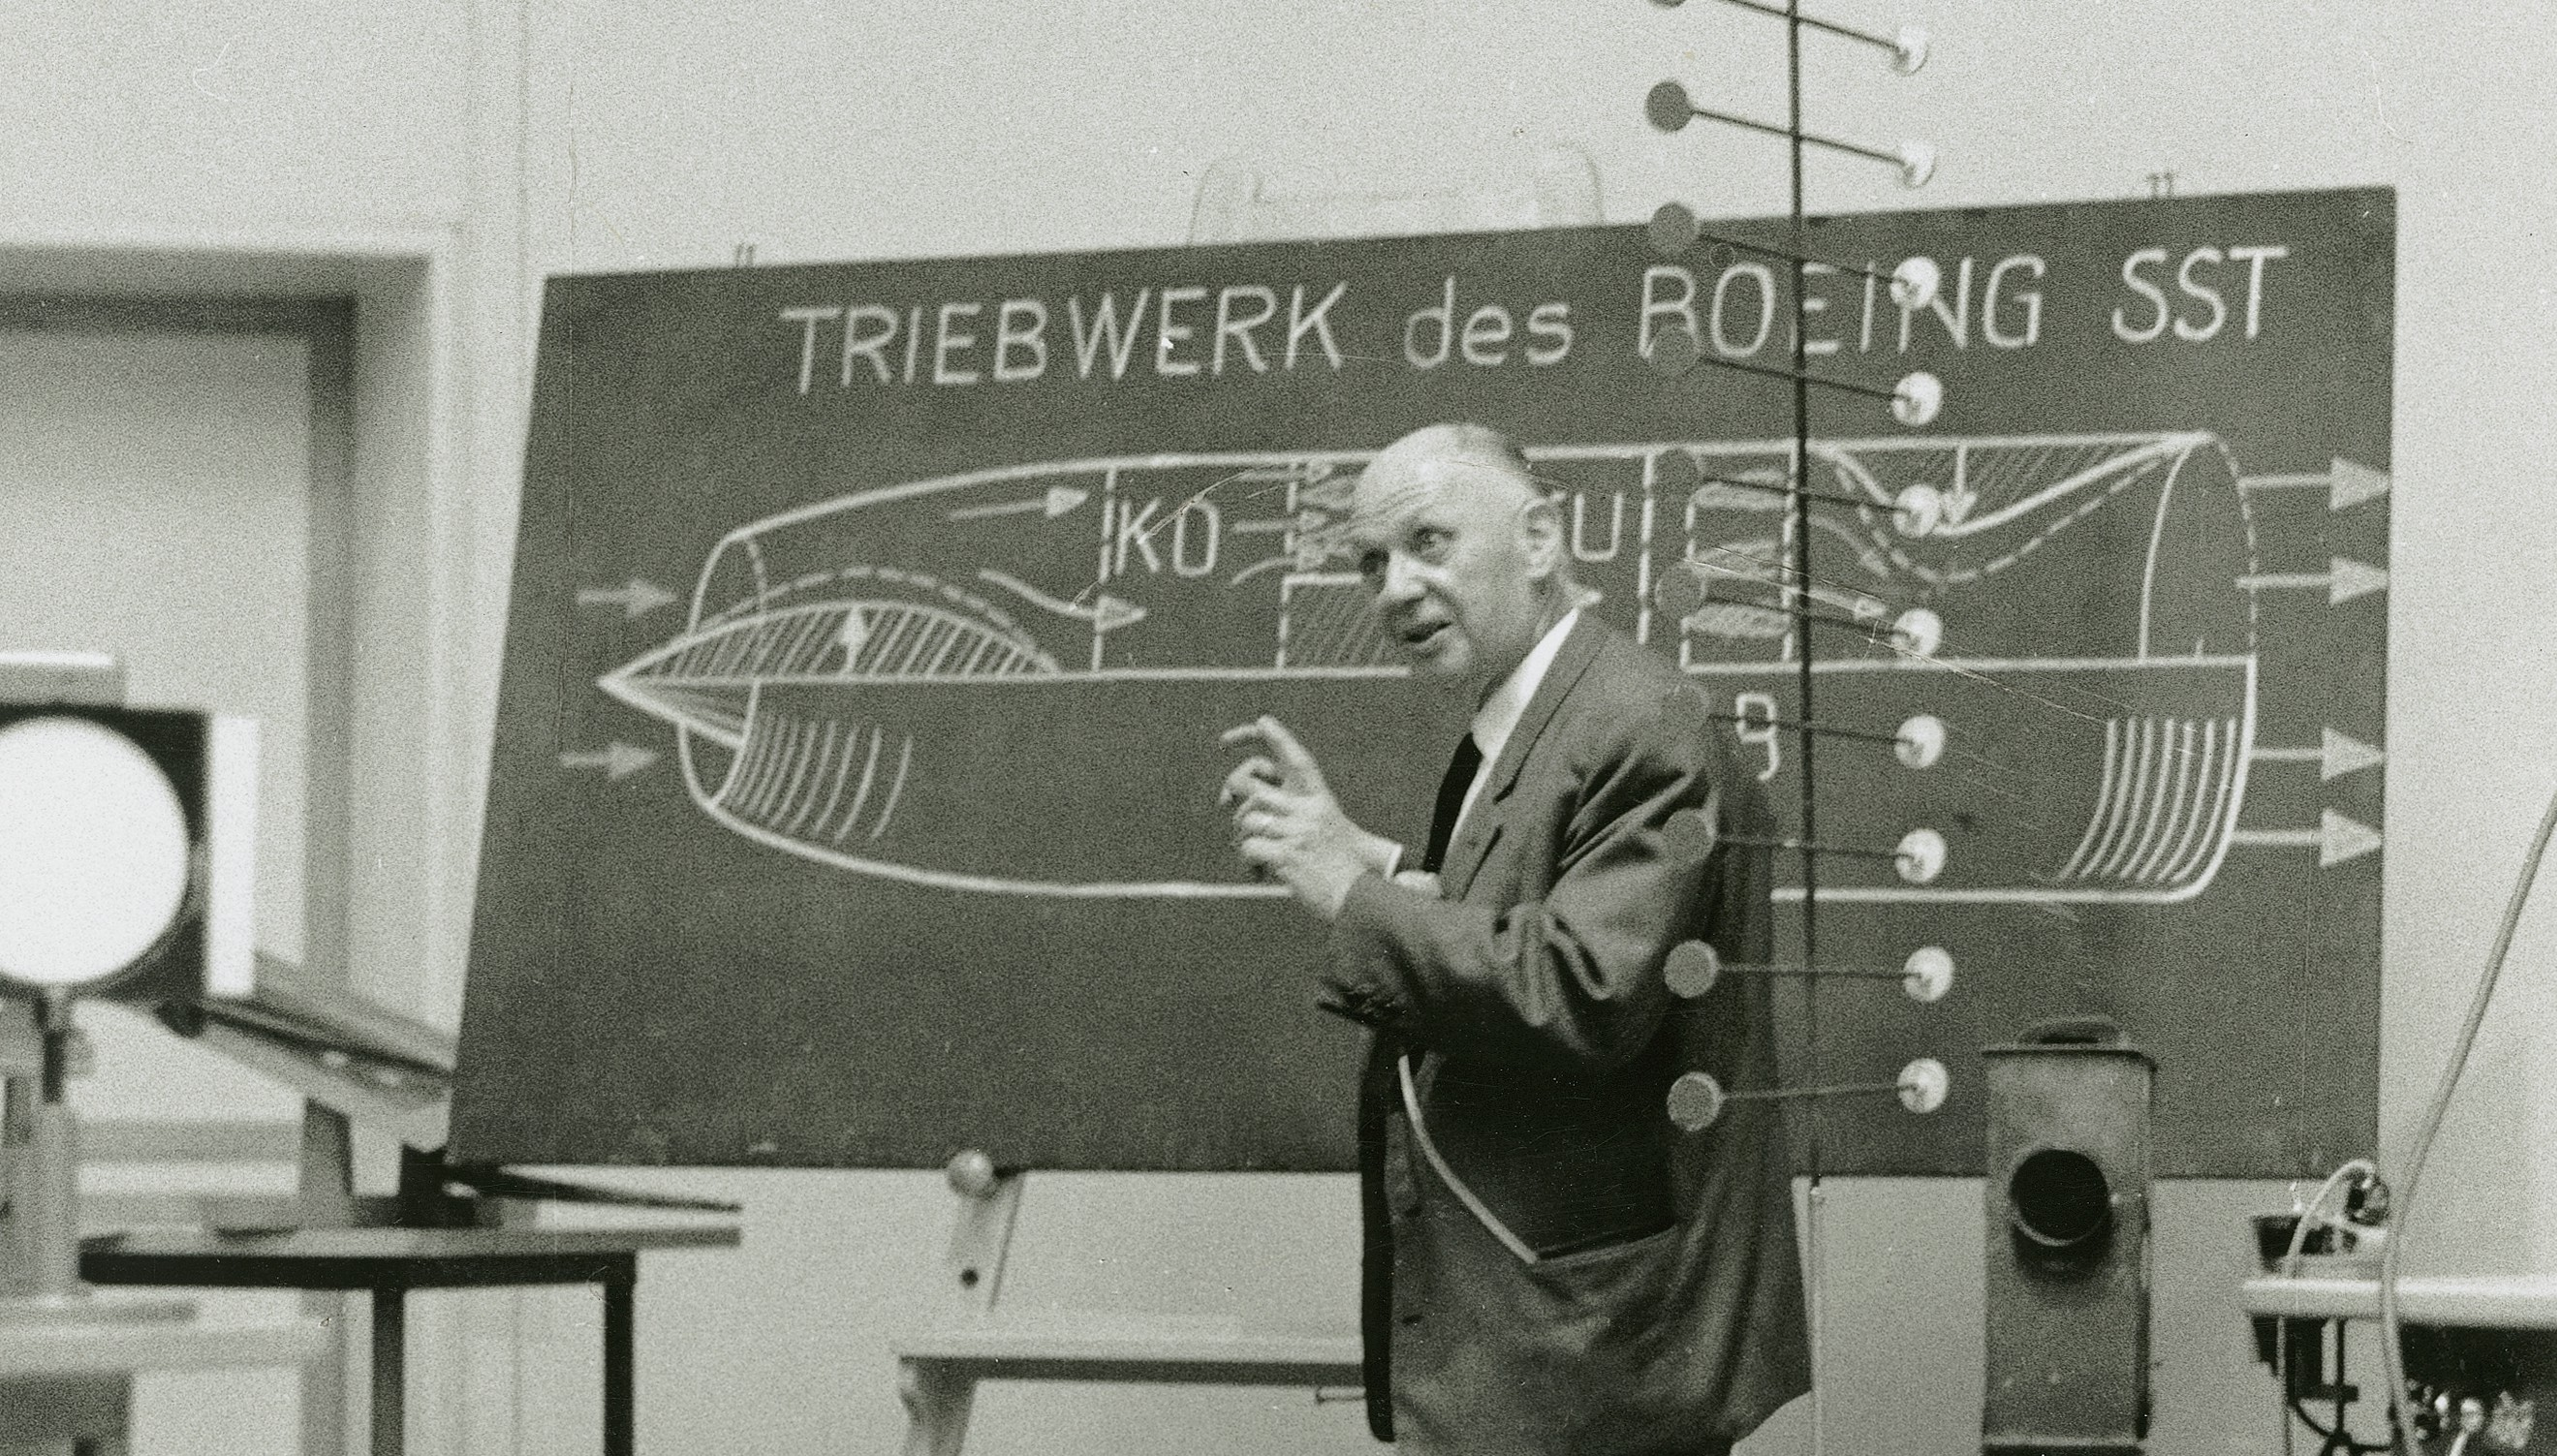
\includegraphics[width=\textwidth]{papers/ueberschall/figures/Jakob_Ackeret_1967.jpg}
    \caption{Professor Jakob Ackeret bei seiner Abschiedsvorlesung~\cite{AckeretFoto1967}.}
    ~\label{fig:ackeret}
\end{figure}
Dort konstruierte er den weltweit ersten 
Überschallwindkanal mit geschlossenem Kreislauf, 
siehe Abbildung~\ref{fig:windkanal}.
Diese Pionierleistung stellte einen bedeutenden 
Meilenstein in der Entwicklung der Überschallluftfahrt dar.
\index{Uberschallluftfahrt@Überschallluftfahrt}%
\begin{figure}
    \centering
    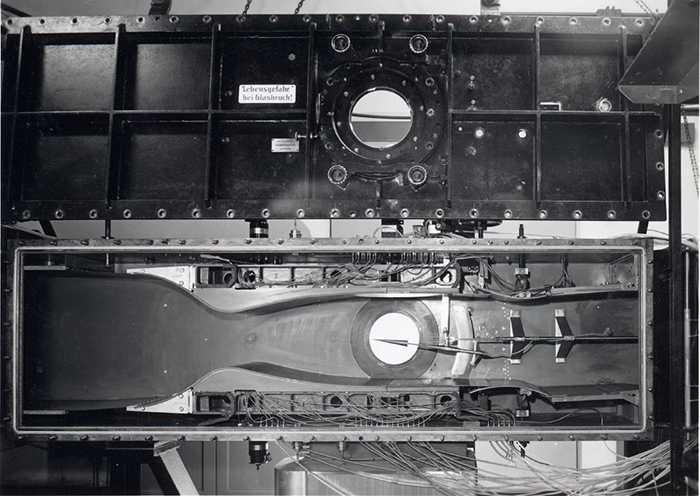
\includegraphics[width=\textwidth]{papers/ueberschall/figures/Windkanal.jpg}
    \caption{Der erste Überschallkanal mit geschlossenem Kreislauf~\cite{ETHeritage2020}.}
    ~\label{fig:windkanal}
\end{figure}

Die Gleichungen der Überschallströmung fanden später 
unter anderem Anwendung bei der Suche nach Körperformen 
mit minimalem Luftwiderstand im Überschallbereich, 
etwa dem sogenannten Sears-Haack-Körper.
Dieser Fragestellung wurde ein ganzes Werk gewidmet,
insbesondere der Beitrag von Carlo Ferrari mit dem Titel 
\index{Ferrari, Carlo}%
\textit{Bodies of Revolution Having Minimum Pressure Drag}~\cite{Ferrari1965}.

